\documentclass[10pt,showpacs,preprintnumbers,footinbib,amsmath,amssymb,aps,prl,twocolumn,groupedaddress,superscriptaddress,showkeys]{revtex4-1}
\usepackage{graphicx}
\usepackage{float}
\usepackage{dcolumn}
\usepackage{bm}
\usepackage[colorlinks=true,urlcolor=blue,citecolor=blue]{hyperref}
\usepackage{color}
\usepackage{listings}

\newcommand{\deriv}[3][]{% \deriv[<order>]{<func>}{<var>}
	\ensuremath{ \frac{d^{#1} {#2}}{d {#3}^{#1}} } }


\begin{document}
\title{Building and effective field theory for neutron-proton scattering}
\author{Thomas Redpath and Dayah Chrisman}
\affiliation{Department of Physics, Michigan State University}
\begin{abstract}

We build an effective field theory (EFT) to describe neutron-proton scattering. We take the
underlying theory to be a sum of three Yukawa potentials with empirically derived parameters
(the potential model from the previous project). By fitting to the low energy phase shifts
($\delta _0$) calculated from solving the Lippman-Schwinger equation, we determine the
coefficients for the contact interactions in the EFT potential. ...


\end{abstract}
\maketitle

\section{Introduction}

Measuring the final states of two nucleons after they interact provides information about
the nature of their interaction. One way to summarize the information we get from these
scattering experiments is through the phase shift - which can be roughly described as a
shift in the scattered wavefunction relative to the incoming one. In this project, we study
the behavior of the $l=0$ phase shift ($\delta _0$) as a function of energy for a toy
neutron-proton ($np$) interaction model.

Qualitatively, we say that a repulsive potential will result in a negative
phase shift - the scattered wavefunction is ``pushed out'' and that an attractive potential
will give a positive phase shift. Thus by analyzing experimental data we can deduce whether
a potential is repulsive, attractive, or a mixture of both. The nuclear potential is negligible at
long ranges ($r >$ a few fm), attractive at intermediate ranges ($r \sim 1$ fm) and repulsive
at very short distances ($r < 0.5$ fm). By examining the phase shift as a function of energy,
we can see at which energies the incoming particle is ``repelled'' (giving a negative phase
shift). This can give us an idea of the range of the repulsive inner part of the potential, since
the particle needs enough energy to approach the inner, repulsive part of the potential.

We organize this report as follows: first we summarize the algorithms we need to solve the
problem numerically. We then describe the framework we used to carry out our calculations.
Next, we present the results of our calcuations and some qualitative insights derived from
considering the variable phase approach. Finally, we summarize our findings and offer some
comments about possible extensions of our framework.



\section{Theory and algorithms}\label{sec:theory}

\subsection{Pionless EFT}

To begin building our pionless effective field theory, we take our underlying theory, to be
the three-Yukawa $np$ model from the previous project. This potential is spin- and
isospin-independent, so the leading order term in the EFT potential has the simple form

\begin{equation}
	V^\mathrm{LO}_{^1S_0}(p',p)=C_0.
\end{equation}

To avoid UV divergences when solving the Lippman-Schwinger equation with this potential,
we use a smooth regulator function

\begin{equation}
\begin{split}
	f_{\Lambda}(p) = \exp{[-p^4/\Lambda^4]}
\end{split}
\end{equation}
so that the potential we feed into our LS solver has the form


\begin{equation}
\begin{split}
	V(p',p)\Rightarrow f_{\Lambda}(p')V(p',p)f_{\Lambda}(p).
\end{split}
\end{equation} 



We start out choosing our cutoff to be $k\sim m_{\pi}/2$, and fit $C_0$ to the low-energy
phase shifts. We then add the next-to-leading-order term (NLO):

\begin{equation}
\begin{split}
%\[
V^\mathrm{NLO}_{^1S_0}(p',p)=C_2(p^2 + p'^2),
%\]
\end{split}
\end{equation}

And subsequently the next-to-next-to-leading-order term (NNLO):

\begin{equation}
\begin{split}
%\[
V^\mathrm{NNLO}_{^1S_0}(p',p)=C_4(p^4 + p'^4) + C'_4 p^2p'^2,
%\]
\end{split}
\end{equation}

After fitting these four coefficients, we repeat the NLO pionless EFT fitting procedures
with different cutoff momenta $\Lambda$ to examine cutoff dependence of our phase
shift calculations.

Finally, we add in a one-pion exchange term in order to create an EFT that works at
higher energies, with a cutoff now at $k\sim m_{\pi}$ . We use a simple toy model
(no spin or isospin dependence) to include one pion exchange: 

\begin{equation}
\begin{split}
%\[
V^\mathrm{LO}(p,p')= V_{\pi}(p,p') + C_0\,
%\]
\end{split}
\end{equation}
while at NLO our potential takes the form
\begin{equation}
\begin{split}
%\[
V^\mathrm{NLO}(p,p')= V_{\pi}(p,p') + C_0 + C_2(p^2+p'^2)\,,
%\]
\end{split}
\end{equation}

We now refit the phase shifts at low energy to find $C_0$ and $C_2$ for out EFT including pions.

\subsection{Least-Squares Fitting}

We use a least-squares fit method to find the coefficients for our EFT. We use $\chi^2$ as a
measure of the quality of the fit, which we aim to minimize the following quantity with respect
to the fitting parameters, $a$ and $b$.
\begin{equation}
\begin{split}
	\chi^2=\sum_{n=1}^{\infty} [y_i-f(x_i,a,b)]/\sigma_i^2
\end{split}
\end{equation}
The hitch of this fitting procedure, though, is that you need a starting point for the parameters
$a$ and $b$ that is roughly close to a $chi^2$ minimum, or your search grid must be very large.

In the case of our EFT, we are using an expansion for the potential that we know hold up at low
momentum. So our LO term should have the largest contribution. It is helpful, then, to start our
search in just one dimension, since each parameter has it's own $\chi^2$ relationship. We fit for
$C_0$ first, and use this local $chi^2$ minimum value to guide our efforts with the NLO and
NNLO coefficients. In this way, we build our EFT to recreate the baseline phase shifts we
calculated in Project 1. 





%\[
%\begin{bmatrix}
%	d_1 & a_1 & 0 & \dots & \dots & 0 \\
%	c_1 & d_2 & a_2 & 0 & \dots & 0 \\
%	0 & c_2 & d_3 & a_3 & 0 & \dots \\
%	\vdots & & \ddots & \ddots & \ddots & \vdots \\
%	\vdots & & & c_{n-2} & \ddots & a_{n-1}\\
%	0 & & & & c_{n-1} & d_n \\
%\end{bmatrix}
%~
%\begin{bmatrix}
%	u_1\\
%	u_2\\
%	u_3\\
%	u_4\\
%	\vdots\\
%	u_n\\
%\end{bmatrix}
%~
%=
%~
%\begin{bmatrix}
%	f_1\\
%	f_2\\
%	f_3\\
%	f_4\\
%	\vdots\\
%	f_n\\
%\end{bmatrix}
%\]

\section{Methods}

We use the low-energy phase shifts from project 1 to fit our parameters in order to create our EFT. 
To calculate phase shifts, we implemented our numerical solution to the Lippman-Schwinger equation
as a \texttt{C++} class. This class consists of three two-dimensional data structures to hold the
$V$, $A$ and $R$ matrices, two one-dimensional data structures to hold the weights and momentum
mesh points that define the integration domain and several ancillary variables that specify the nucleon
mass and other book-keeping parameters. Application of the algorithms sketched in the previous
section is carried out in a series of member functions that (a) set up the mesh points and weights (b)
set up the potential matrix (c) set up the $A$ matrix (d) invert $A$ to get $R$ then extract $\delta _0$. 

This class is defined in the source
files \texttt{NucleonScattering.cpp} and \texttt{NucleonScattering.hh}. An instance of the class is
created and the correct sequence of methods is called in the \texttt{main} function defined in
\texttt{main.cpp}.

For our benchmark data, we use an NP potential with the form

%put NP potential here!!!


and calculate the phase shifts for a range of energies.
We then use our LO, NLO, and NNLO EFT potentials from above to calculate the phase shifts for 
a range of energies. Since we know the form of the potential, we can use a last-squares fitting procedure to get values for our LO, 
NLO, and NNLO coefficients. This procedure is outlined above in the Theory section.

%specify chi^2 space searh procedure here!!! i.e. did we search the full 4 dimensional space or look around the chi^2 minimum for C_0 to find the others?


%% -------------------------- CODE LISTING -------------------------- %%

%% 
 \definecolor{mygreen}{rgb}{0,0.6,0}
 \definecolor{mygray}{rgb}{0.5,0.5,0.5}
 \definecolor{mymauve}{rgb}{0.58,0,0.82}

 \lstset{ %
   backgroundcolor=\color{white},   % choose the background color; you must add \usepackage{color} or \usepackage{xcolor}
   basicstyle=\footnotesize,        % the size of the fonts that are used for the code
   breakatwhitespace=false,         % sets if automatic breaks should only happen at whitespace
   breaklines=true,                 % sets automatic line breaking
   captionpos=b,                    % sets the caption-position to bottom
   commentstyle=\color{mygreen},    % comment style
   deletekeywords={...},            % if you want to delete keywords from the given language
   escapeinside={\%*}{*)},          % if you want to add LaTeX within your code
   extendedchars=true,              % lets you use non-ASCII characters; for 8-bits encodings only, does not work with UTF-8
   frame=single,	                   % adds a frame around the code
   keepspaces=true,                 % keeps spaces in text, useful for keeping indentation of code (possibly needs columns=flexible)
   keywordstyle=\color{blue},       % keyword style
   language=C++,                 % the language of the code
   otherkeywords={*,...},           % if you want to add more keywords to the set
   numbers=left,                    % where to put the line-numbers; possible values are (none, left, right)
   numbersep=5pt,                   % how far the line-numbers are from the code
   numberstyle=\tiny\color{mygray}, % the style that is used for the line-numbers
   rulecolor=\color{black},         % if not set, the frame-color may be changed on line-breaks within not-black text (e.g. comments (green here))
   showspaces=false,                % show spaces everywhere adding particular underscores; it overrides 'showstringspaces'
   showstringspaces=false,          % underline spaces within strings only
   showtabs=false,                  % show tabs within strings adding particular underscores
   stepnumber=2,                    % the step between two line-numbers. If it's 1, each line will be numbered
   stringstyle=\color{mymauve},     % string literal style
   tabsize=2,	                   % sets default tabsize to 2 spaces
   title=\lstname                   % show the filename of files included with \lstinputlisting; also try caption instead of title
 }

 %\lstinputlisting[linerange={78-90}]{../src/proj1.cc}


%\begin{figure*}
%	\includegraphics[width=\textwidth]{figures/stability.pdf}
%	\caption{Results for the finite square well ($V_0 = -0.5$ fm$^2$, $a = 1.$ fm) $l=0$
%	phase shifts  as a function of lab energy. In each plot, our calculations are represented by the
%	blue points and the analytic results are plotted in red. The black points in the lower plots
%	show the deviation of our calculation from the analytic result. From left to right we plot the
%	results of our calculation for N=5, N=50 and N=100 to show convergence for 50 mesh points.}
%	\label{fig:analyticDelta}
%\end{figure*}


\section{Results and discussion}

\subsection{Pionless EFT}
We began our EFT with the leading order term for the potential
\begin{equation}
\begin{split}
V^\mathrm{LO}_{^1S_0}(p',p)=C_0.
\end{split}
\end{equation}
We calculated the phase shifts for various values of $C_0$, and plotted them against the
$\chi^2$ value for the comparison to our benchmark data from Project 1. 


We then picked out the value of $C_0$ for which $\chi^2$ is a minimum, and calculated
the phase shifts for the LO potential.

Our results agree at low lab energy (low-momentum), which we expect due to our expansion. 

Next, we added the next-to-leading-order term to our potential

\begin{equation}
\begin{split}
V^\mathrm{NLO}_{^1S_0}(p',p)=C_2(p^2 + p'^2),
\end{split}
\end{equation}

This time, we initialized $C_0$ at the value found from the leading-order fit. We plotted
$\chi^2$ in both dimensions to visually pick out a local minimum around which to search,
and to get an idea of a reasonable threshold for acceptance.

\subsection{Including One-Pion Exchange}


%%%%%%%%%%%%%%%%%
%%%%% Pionless figures %%%%%
%%%%%%%%%%%%%%%%%

\begin{figure}
\centering
	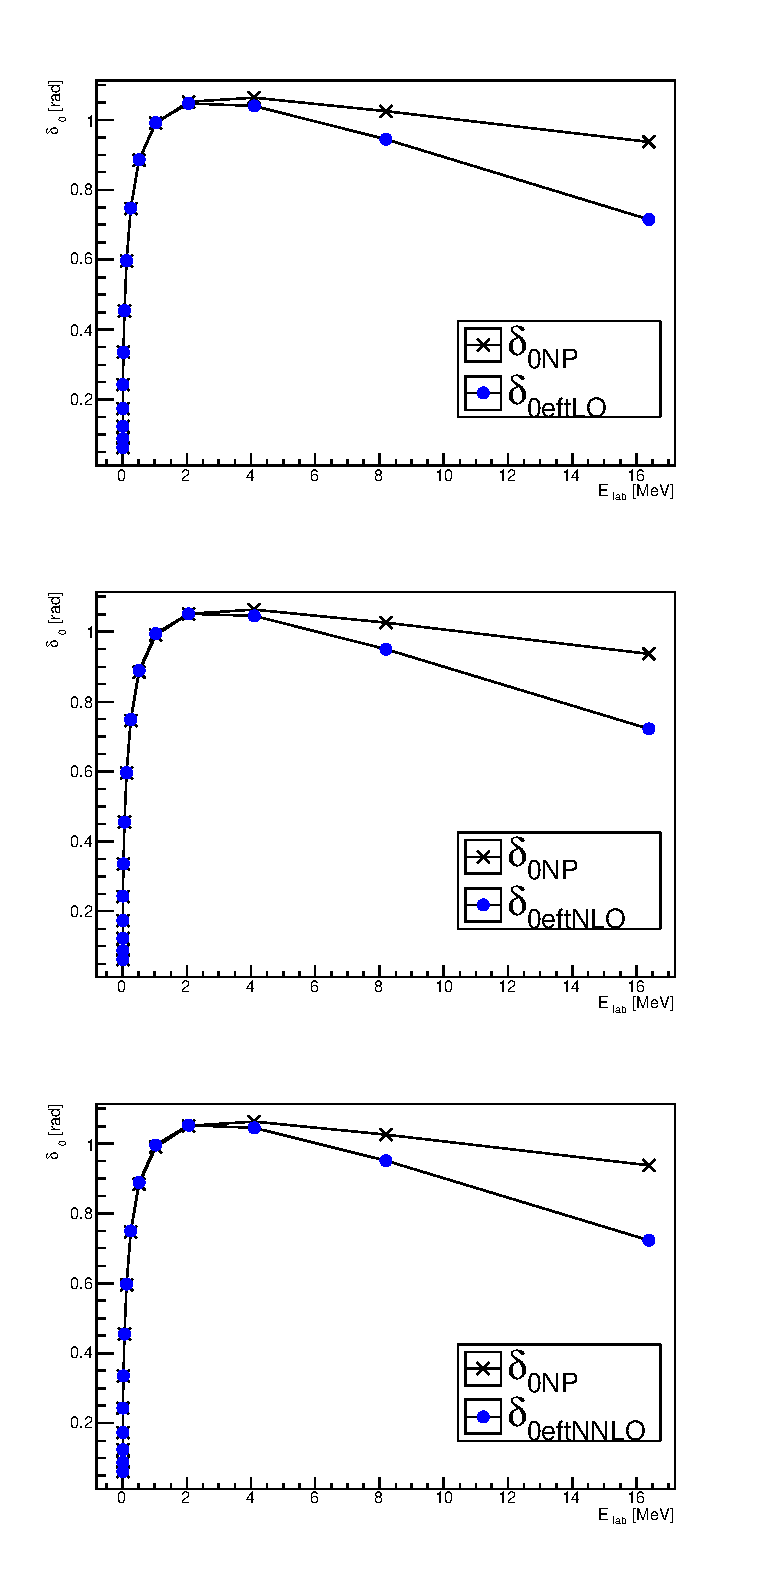
\includegraphics[width=0.5\textwidth]{figures/phy989_pionless.eps}
	\caption{Comparison between the three-Yukawa $np$ model $l=0$ phase shifts
	(black X)
	and the phase shifts calculated from the LO, NLO, NNLO EFT potentials (blue
	dots).}
	\label{fig:pionless}
\end{figure}

\begin{figure}
\centering
	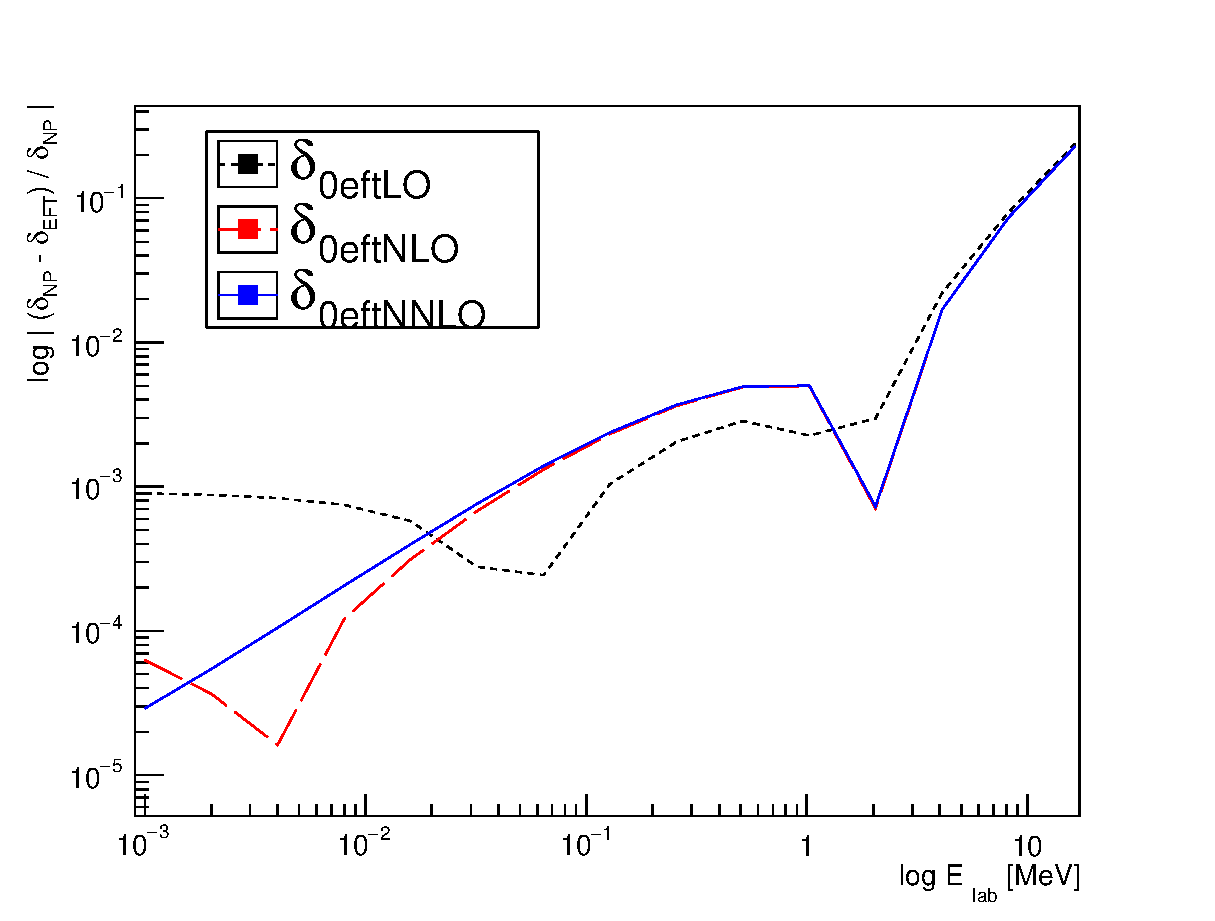
\includegraphics[width=0.5\textwidth]{figures/phy989_pionlessLepage.eps}
	\caption{Lepage error plot comparing the LO, NLO, NNLO EFT potentials to the
	$np$ model pseudo data. The kinks in the lines are where the sign of the error
	changes. The NLO and NNLO errors are the same above lab energies of 100
	keV.}
	\label{fig:pionlessLepage}
\end{figure}

\begin{figure}
\centering
	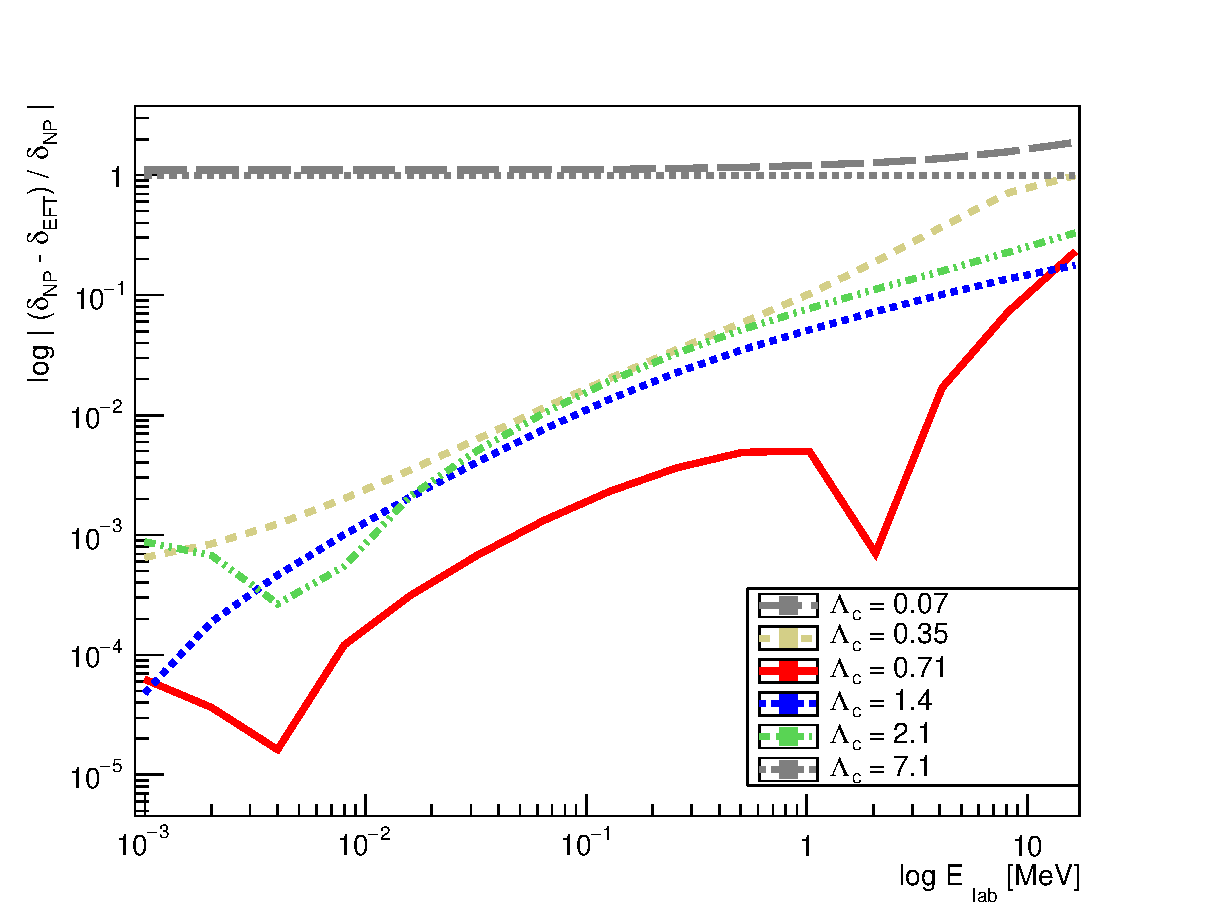
\includegraphics[width=0.5\textwidth]{figures/phy989_pionlessCutoff.eps}
	\caption{Lepage error plot for NLO EFT potentials with various cutoffs $\Lambda_c$.
	From these results, we deduce that $\Lambda_c = 0.71$ (the pion mass) is roughly
	the breakdown scale for which setting $\Lambda_c$ too far below or above this
	value worsens the agreement with the underlying theory.}
	\label{fig:LepageCutoff}
\end{figure}

\clearpage

%%%%%%%%%%%%%%%
%%%%% PIONS !!! %%%%%
%%%%%%%%%%%%%%%

\begin{figure}
\centering
	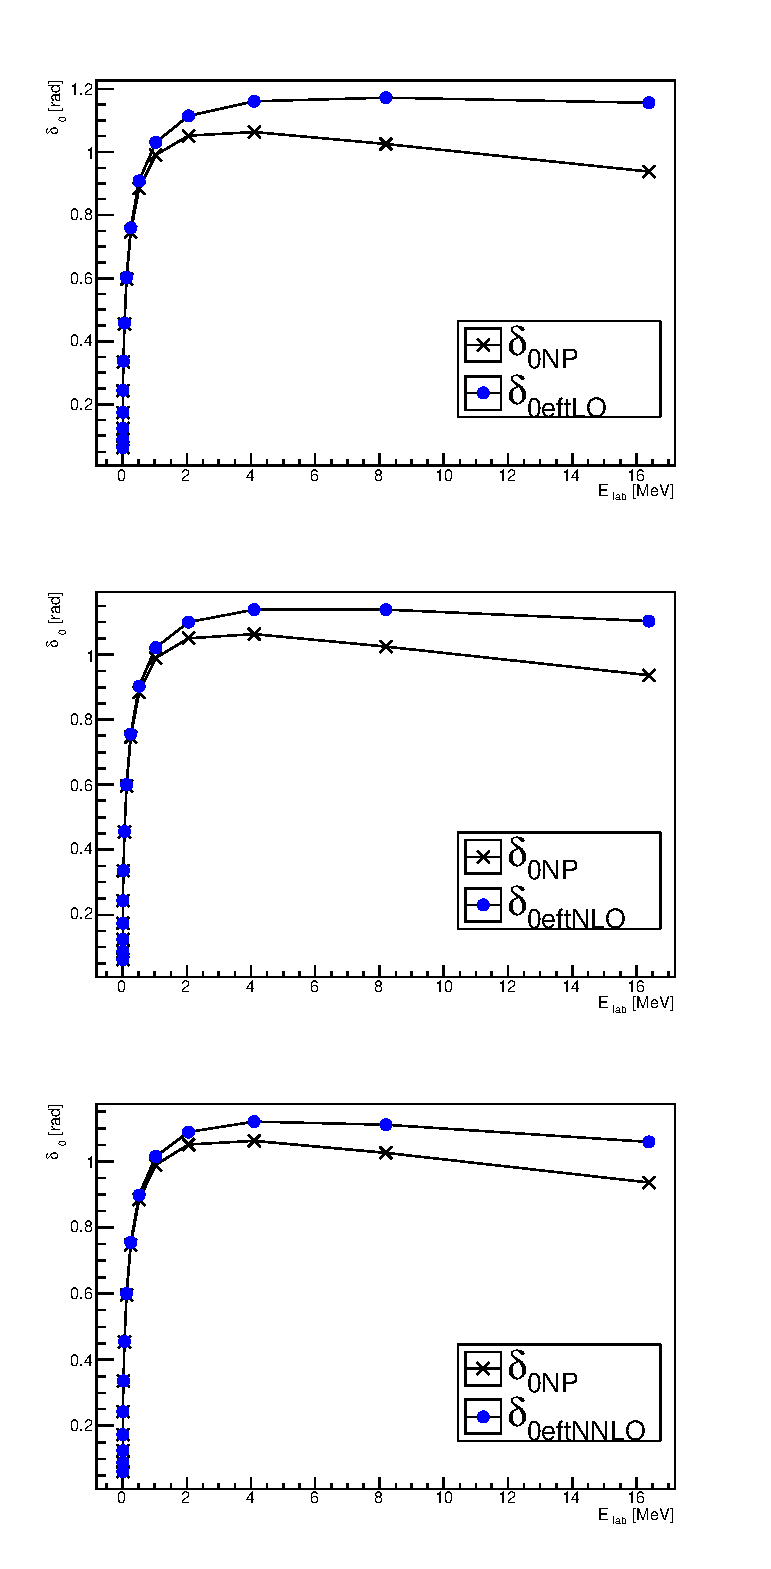
\includegraphics[width=0.5\textwidth]{figures/phy989_OnePion.eps}
	\caption{Comparison between the three-Yukawa $np$ model $l=0$ phase shifts
	(black X)
	and the phase shifts calculated from the LO, NLO, NNLO one-pion exchange
	EFT potentials (blue dots).}
	\label{fig:OnePion}
\end{figure}

\begin{figure}
\centering
	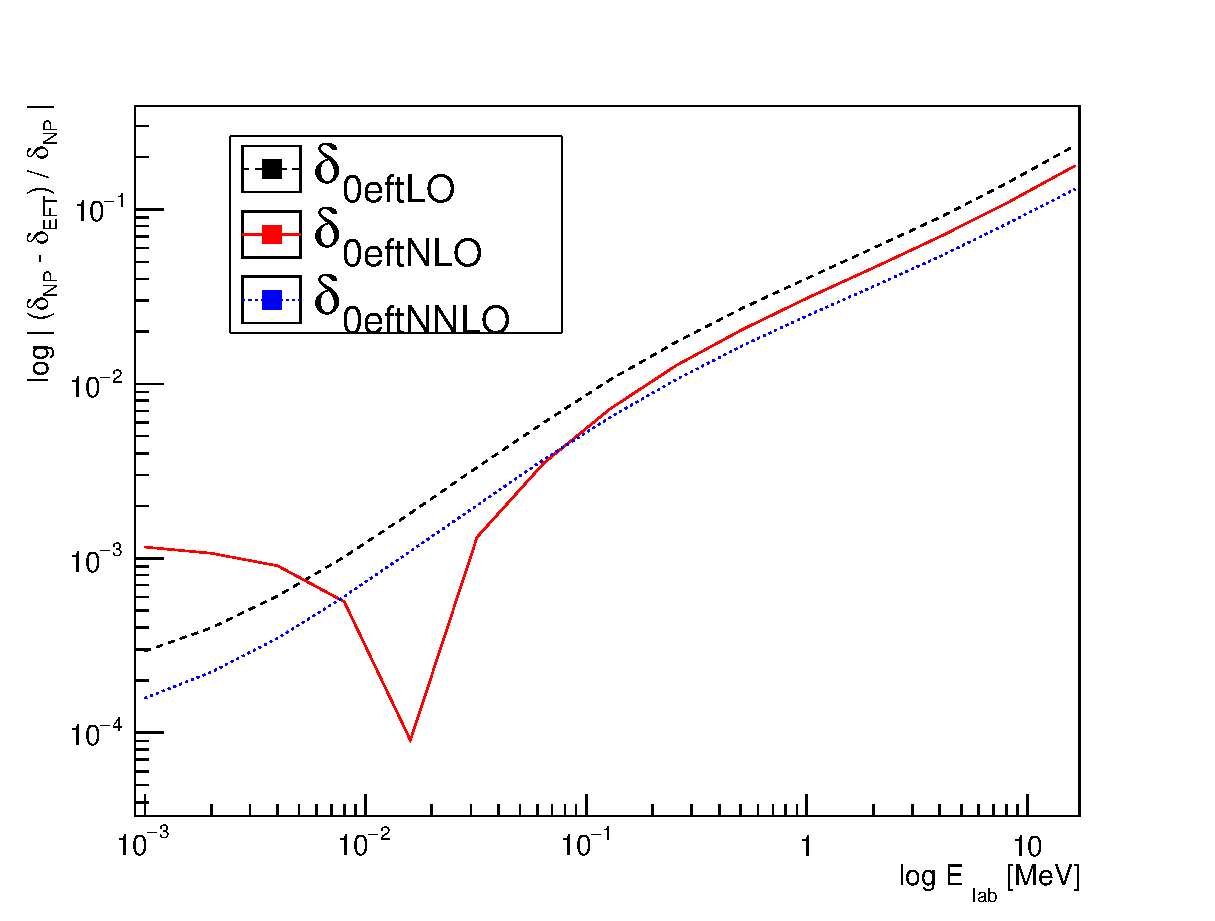
\includegraphics[width=0.5\textwidth]{figures/phy989_OnePionLepage.eps}
	\caption{}
	\label{fig:OnePionLepage}
\end{figure}

\begin{figure}
\centering
	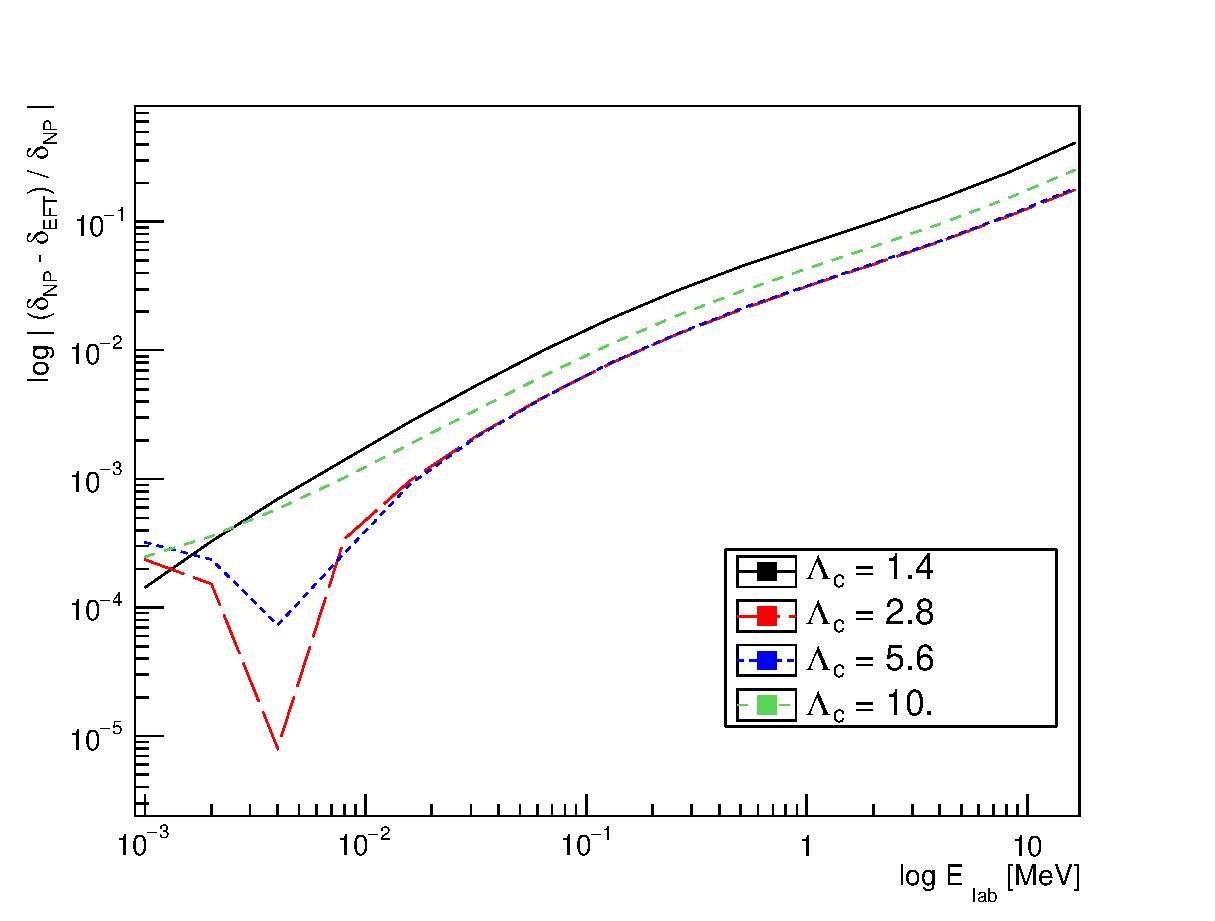
\includegraphics[width=0.5\textwidth]{figures/phy989_OnePionCutoff.eps}
	\caption{Lepage error plot comparing the $np$ model and EFT $\pi-$NLO with
	for various cutoff values $\Lambda_c$.}
	\label{fig:OnePionCutoff}
\end{figure}


\section{Conclusions}

A more rigorous fitting routine would do a better job of tuning the EFT coefficients.


%\begin{thebibliography}{99}
%\bibitem{miller2006} G.~A.~Miller, A.~K.~Opper, and E.~J.~Stephenson, Annu.~Rev.~Nucl.~Sci.~{\bf 56}, 253 (2006).
%\bibitem{Morten} M. Hjorth-Jensen, Computational Physics Lecture Notes Fall 2015, August 2015.
%\bibitem{Mslides} M. Hjorth-Jensen, Computational Physics Notes, compphysics.github.io
%\bibitem{Golub1996} G. Golub, C. Van Loan, \textit{Matrix Computations} (John Hopkins University Press, 1996)
%\end{thebibliography}

\bibliographystyle{plainnat}
\bibliography{refs}

\end{document}
